% \documentclass[preprint]{kcc}
\documentclass{kcc}


%%%%%%%%%%%%%%%%%%%%%%%%%%%%%%%%%%%%%%%%%%%%%%%
% include additional packages you need to use
%%%%%%%%%%%%%%%%%%%%%%%%%%%%%%%%%%%%%%%%%%%%%%%
% graphic, float package
\usepackage{graphicx}		% for setting images
\usepackage{float}			% for float objects
\usepackage{subfigure}	% for adding several figures in a figure environment
\usepackage{lscape}			% for landscape type images or tables

% Reduce the line spacing in the bibliography
\let\oldbibliography\thebibliography
\renewcommand{\thebibliography}[1]{%
  \oldbibliography{#1}%
  \setlength{\itemsep}{0pt}%
}

\usepackage{enumitem}

% for compact section title spacing
% \usepackage[compact]{titlesec}

% nameref
\usepackage{nameref}

% mathmetical presentation
\usepackage{gensymb}
\usepackage{amsmath}
\usepackage{dsfont}
\usepackage{amssymb}
\usepackage{amsthm}
\usepackage{exscale}
\usepackage{textcomp}		% extra symbols


% for circled number
\newcommand{\cl}[1]{\textcircled{\scriptsize #1}}


% package for using algorithmic presentation
\usepackage{algorithmic}
\usepackage{algorithm}
% customize algorithmic environment
\renewcommand{\algorithmicrequire}{\makebox[40px]{\hfill\textbf{Input :}}}
\renewcommand{\algorithmicensure}{\makebox[40px]{\hfill\textbf{Output :}}}

\DeclareMathOperator*{\argmin}{\arg\!\min}
\DeclareMathOperator*{\argmax}{\arg\!\max}

% array and table presentation
\usepackage{array}
\usepackage{tabulary}
\usepackage{multirow}
\usepackage[table]{xcolor}
\usepackage{ctable}
\usepackage{booktabs}		% for typesetting tables at the level of publication
							          % do not use vertical rule
\usepackage{lipsum}
							
% set title, author, abstract
\title{시선 정보를 이용한 만화 영상의 가속화된 선택적 학습 방법}
\author{
}
\engtitle{Accelerated Selective Learning from Cartoon Videos with Eye-Gaze Information}
\engauthor{
}
\abstract{
기계 학습에서 GPU를 이용할 수 있게 되면서 대용량 이미지 데이터를 효과적으로 다룰 수 있었다. 그러나 많은 선행 연구에서 영상 데이터를 학습 대상으로 삼을 때 계산적 비용과 일반적인 연구실 환경의 물리적 한계로 그 연구의 넓이가 제한되었다. 본 연구는 약 100시간 분량의 영상 데이터를 한 대의 서버에서 학습하는 방법을 제안한다. 하정우 외 (2015)의 깊은 개념 층(DCH) 모델에서 시각 정보의 선택적 학습을 그래프 몬테 카를로(Graph Monte Carlo)를 이용하여 수행할 때, 1시간 분량의 영상 정보에 대하여 수집 된 다수 사람의 시선 분포 정보를 이용함으로써 선택적 학습을 가속화 시킨다. 이때 컨볼루션 네트워크로 학습한 일부 영상 구간의 시선 분포를 전체 구간으로 일반화하여 적용 가능한지 살펴본다.
}

\begin{document}

\maketitle


\section{서 론}
전통적으로는 멀티 코어 프로세서를 이용한 병렬 처리 부터 데이터 센터의 광 네트워크를 이용한 클라우딩 컴퓨팅을 사용하는 방법을 이용하여 계산 시간적 비용을 줄이는 방법을 택하였다. 그러나 최근 그래픽스 산업계에서 GPU를 이용한 라이브러리를 제공하는 등의 지원을 통해 GPU를 이용한 기계 학습이 보편화 되고 있다. 현재는 보급형 그래픽 카드에서도 CPU의 400배 이상의 코어를 제공하는데 온 칩 메모리와 프로세서 간의 짧은 대기 시간 이용하여 상대적으로 저렴해진 실험 환경 구축 비용으로 많은 데이터를 처리할 수 있게 되었다.

이러한 혜택을 가장 크게 받은 영역은 이미지 데이터 였다. 최근의 이미지 분류 문제에서 GPU 계산을 이용하지 않고는 궁극적으로 모델의 학습 시간이 일반적인 학술대회 개최 주기인 1년 보다 길어질 수 있기 때문에 최고 수준의 성능의 연구 성과를 발표하기 어렵게 되었다. 현재 가장 큰 데이터인 ImageNet의 경우 최고 수준의 성능을 보이는 모델은 1주 정도의 학습 기간이 요구되고 있다 \cite{krizhevsky2012imagenet}.

하지만 최근 인공지능 연구는 이미 사람과 유사한 성능을 보이고 있는 물체 인식 문제를 넘어 둘 이상의 양태나 시간 정보를 기반으로 하는 다양한 데이터에서 인지 모델을 구축하기 위한 노력을 하고 있다. 특히 하정우 등 \cite{zhou2006learning}\cite{Ha2015}의 연구에서는 만화 영상을 통한 상호적 기반의 시각-언어 개념 학습 모델인 깊은 개념 층(DCH)을 제시한다. 이 모델은 언어의 기반이 같은 양태인 언어에만 국한된 것이 아니라 정보적으로 연관된 시각 정보에도 기반을 두고 있으며, 그 반대로 시각 정보 역시 정보적으로 연결된 언어에 기반하여 개념을 형성한다는 주장을 제안하는 모델과 함께 보였다. 

DCH 모델은 다양한 문제 상황에서 객체들 간의 관계를 학습하기 위해 연구되고 있는 하이퍼그래프를 사용하는데 \cite{zhou2006learning}, 구체적으로는 시각 정보로 만화 영상 이미지에서 추출한 SIFT 특징 벡터를, 언어 정보는 만화 영상의 영어 자막 텍스트를 이용하였다. 만화 영상의 에피소드가 재생되는 순서에 따라 자막이 나타나는 시점을 기준으로 그래프 몬테 카를로(Graph Monte Carlo)를 이용하여 해당하는 시점의 영상 이미지의 SIFT 특징 벡터들과 자막 텍스트의 단어를 하이퍼그래프의 노드로 샘플링 한다. 이 노드들을 연결하는 하이퍼엣지의 가중치는 모델과 한 양태가 주어졌을 때 다른 양태의 정보를 확률적으로 재생성할 수 있는 목적 함수에 따라 조정 된다. 

우리는 이 방법에서 특히 영상 이미지에서 중요하지 않은 배경 물체에 대한 정보이거나 결과적으로 텍스트와의 상호 정보가 부족한 SIFT 특징 벡터들이 샘플링 대상에 많다는 것에 주목하고, 사람의 안구 운동 측정을 통해 수집한 다수 사람의 시선 분포 정보를 그래프 몬테 카를로 방법에 이용함으로써 선택적 학습을 가속화 시키고자 한다 \cite{Oh2011}. 이 때 컨볼루션 네트워크를 이용하여 영상 정보로부터의 얻은 시각 모델과 사람의 안동 운동에서 관찰된 시선 정보 모델의 차를 적게 하도록 유도하는 목적 함수를 이용함으로써 제한된 시선 분포 정보를 가지고 일반화된 모델을 획득 하고자 한다. 이 논문에서는 다수 사람의 시선 분포 정보를 학습 모델에 적용할 수 있는 이론을 제시하고 시선 분포의 계산학적 특징을 고찰하고자 한다.

따라서, 본 연구는 다음과 같은 두 가지 가설을 검증하고자 한다. i) 컨볼루션 네트워크는 영상의 일부에 대한 시선 분포를 학습하여 전체 영상에 적용할 수 있도록 일반화 될 수 있다. ii) 새로운 메타 정보인 학습된 시선 분포를 이용하여 그래프 몬테 카를로 방법을 사용하면 기존 샘플링 방법 보다 좋은 성능을 얻는다.

\section{DHC 모델}

\begin{figure*}
  \centerline{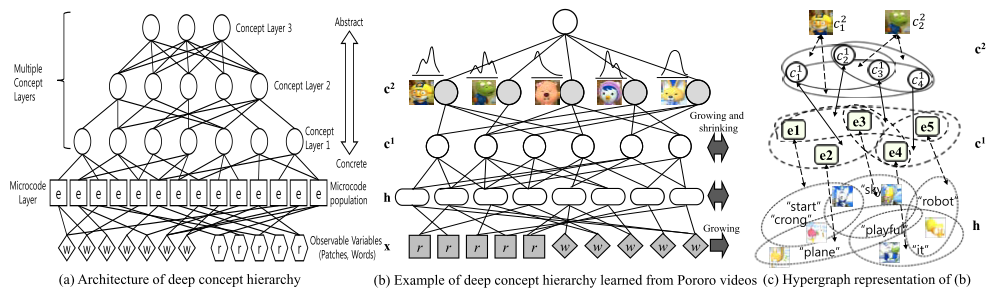
\includegraphics[width=180mm,height=54mm]{eps/ha2015_fig2.png}}
  \caption{DCH 모델의 이론적 개념도. (a)는 DCH의 계층 구조를 보여주며, (b)는 두 개의 개념 계층 망을 가지고 뽀로로 만화 영상에 대한 개념도를, (c)는 (b)에 대한 하이퍼그래프 표상을 나타낸다. (b)에서 c2는 지도 학습 목표가 되는 캐릭터 등장 라벨을, r과 w은 데이터에서 관찰된 값을 나타내며, r은 이미지 특징 벡터에 대한 노드를, w는 자막 텍스트에 대한 노드를 나타낸다. 모델에 대한 이해를 돕기 위해 저자의 동의를 얻어 본 논문에 포함하였다 \cite{Ha2015}.}
  \label{fig:ha2015}
\end{figure*}

DHC 모델은 점진적으로 들어오는 데이터를 그래프 몬테 카를로 방법한 샘플링 방법으로 데이터와 더불어 점진적으로 하이퍼그래프를 구축한다. $G^{*}$를 최적의 하이퍼그래프라고 둘 때 베이지안 법칙에 의하여 아래과 같이 표현될 수 있다.

\begin{equation} \label{eq1}
\begin{split}
G^{*} & = \argmax_{G_{t}} P(G_{t}|D) \\
      & = \argmax_{G_{t}} P(D|G_{t})P(G_{t-1}) \\
\end{split}
\end{equation}

이 모델은 각 영상 이미지에 등장하는 캐릭터를 나타내는 지표 벡터 $y \in \mathds{R}^{|c2|}$를 이용하여 지도 학습을 하게 된다. 형식적으로 아래와 같이 관찰된 데이터와 캐릭터 지표 벡터를 통해 하이퍼그래프를 구성한다.

\begin{equation} \label{eq2}
\begin{split}
P(G|D,y) & = \frac{P(D|G,y) P(y|G) P_{t-1}(G)} {P(D,y)} \\
\end{split}
\end{equation}

여기서 $P(D|G,y)$는 데이터 재생성 항으로서 모든 하이퍼엣지의 학습된 가중치의 합 대비 데이터에 대하여 연결된 하이퍼엣지 가중치 합의 비율로 정의 되며 softmax 함수, 또는 다른 표현으로, 정규화된 지수 방법을 사용한다. 가중치는 전적으로 관찰(샘플링) 된 데이터의 빈도 수에 따라서만 조정되므로 그래프 몬테 카를로 방법에 따라서 그 성능이 크게 변하게 되며 의존적 이다\cite{zhang1994accelerated,Zhang1998}. 자세한 내용은 하정우 등\cite{Ha2015}의 논문을 참고하길 바란다.

\section{Hybrid 그래프 몬테 카를로}
위의 모델에서 가장 효과적인 그래프 몬테 카를로 방법으로 보상적 그래프 몬테 카를로(FGMC) 방법을 제안 하였다. 이 샘플링 기법은 샘플링이 적게 된 노드를 더 많이 샘플링 되도록 한다. 따라서 시각-언어 번역 테스트에서 정확도는 다른 기법에 비해 소폭 상승하였지만 재현도에서 상대적으로 큰 값을 가졌다. 빈도 수가 상대적으로 작은 특징들에 대해 보다 정확한 경험적 확률 분포를 얻기 위한 방법으로 크고 희소한 그래프를 만들게 됨으로써 비효율적 그래프를 학습하게 된다.

이러한 원인은 그래프 몬테 카를로 방법에 의한 가중치 조정이 추론의 중요한 요인이 됨에도 불구하고 언어 정보를 직접적으로 추론할 수 없는 낮은 수준의 특징 값인 SIFT 특징 벡터들을 샘플링 대상으로 삼기 때문에 효율적인 샘플링을 위한 정보가 부족하다. 본 연구에서는 이러한 언어 정보를 추론하는 데에 도움을 줄 수 있는 1시간 분량의 영상에 대한 다수 사람의 시선 분포 정보를 이용하여 SIFT 특징 벡터들을 샘플링 하는 방법을 제안하고자 한다.

다수 사람의 시선 분포 정보는 모든 데이터 입력에 대한 값을 실험적으로 가지는 것은 비효율적이므로 컨볼루션 신경망(Convolutional Neural Networks)을 이용하여 입력 이미지 $\mathcal{I}$에 대한 분포 추정 값 $\hat{\pi}$을 관찰된 시선 분포 $\pi$를 통해 얻는다. 여기서 컨볼루션 신경망의 마지막 층은 분포에 대한 오차를 에러 함수로 정의한 후 파라미터 값들을 어렵지 않게 학습할 수 있다. $\hat{\pi}$를 이용한 아래의 수식은 기존 연구의 그래프 몬테 카를로 방법으로 치환하게 된다.

\begin{equation} \label{eq3}
\begin{split}
P(v_{i}) & = \frac{\exp(\hat{\pi}(pos(v_{i})) \cdot w_{i} \cdot log(R(d(v_{i}))))}{Z}
\end{split}
\end{equation}

수식~\ref{eq3}에서 함수 $pos(v_{i})$는 노드 $v_{i}$의 이미지 $\mathcal{I}$ 상에서의 위치를, 함수 $d(v_{i})$는 학습된 하이퍼그래프 안에서 연결된 정도(degree), 함수 $R$은 가능한 집합 내 $v_{i}$의 순위를 나타낸다. 순위 값은 로그 크기 조정 후 사용한다. $w_{i}$은 현재 관찰된 빈도 수를 나타낸다. 이미지 $\mathcal{I}$에서 추출한 SIFT 특징 벡터는 클러스터링을 통해 한 노드로 표현되므로 빈도 수가 1 이상일 수 있다. 수식~\ref{eq4}는 총 합이 1이 되게 하는 분모를 나타낸다.

\begin{equation} \label{eq4}
\begin{split}
Z & = \exp(\sum_{i=1}^{|v|}{P(v_{i})})
\end{split}
\end{equation}

\begin{figure}
  \centerline{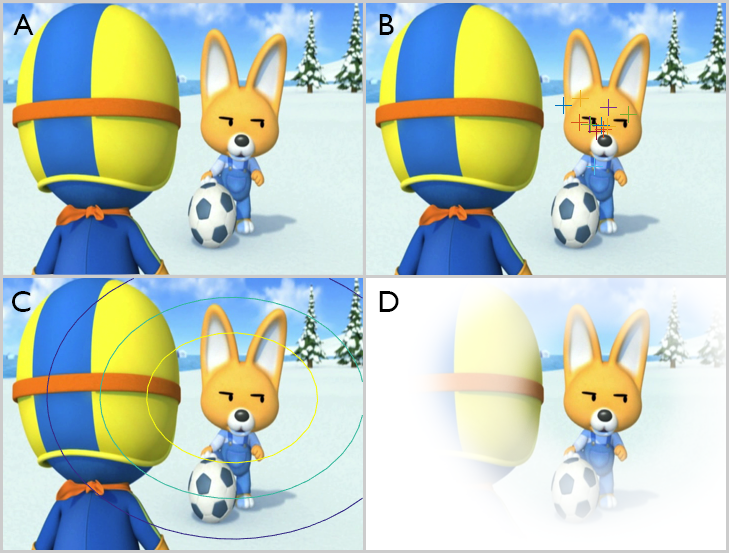
\includegraphics[width=92mm,height=70mm]{eps/sel_fig2.png}}
  \caption{시선 정보를 활용하는 방법을 도식화. A는 원본 이미지, B는 만화 영화 시청 상황에서 A의 이미지에 해당하는 프레임 시각에 응시한 서로 다른 13명의 응시 좌표들을 십자가 기호로 나타내었다. C는 응시 좌표들을 가우시안 혼합 모델(Gaussian Mixture Model)로 나타냈을 때의 확률 분포를 세 개의 등고선으로 어림 표현하였다. D는 그래프 몬테 카를로 방법으로 샘플링할 SIFT 벡터의 확률 가중치를 도식적으로 표현한다. 컨볼루션 네트워크에서 학습할 분포는 C의 분포가 된다.}
  \label{fig:selective}
\end{figure}

\iffalse
\begin{figure}
  \centerline{\includegraphics[width=60mm,height=54mm,trim=65mm 103mm 68mm 100mm]{}}
  \caption{긴 응시와 짧은 응시에 대한 장기 기억 능력 시험 결과 이다. 긴 응시와 짧은 응시에 대한 기억력 점수는 통계적으로 유의미 하지 않았다(p $=$ 0.5051). 오차 막대는 $\pm$ 2 표준 오차를 뜻 한다. 실험에 대한 자세한 설명은 ~\nameref{subsec:experiment2} 소절을 참조한다.}
  \label{fig:memtest-leng}
\end{figure}

\begin{figure}
  \centerline{\includegraphics[width=60mm,height=54mm,trim=55mm 108mm 58mm 105mm]{}}
  \caption{}
  \label{fig:memtest-nested}
\end{figure}
\fi

\section{토 론}

그래프 몬테 카를로를 영상 데이터에 사용하게 된 것은 풀고자 하는 문제가 정확한 객체 인식의 문제에서 정확한 개념 형성의 문제로 치환되었기 때문이다. 객체 인식의 문제에서는 모델 학습이 풀고자 하는 분류의 범위가 고정되고 입력 데이터의 범위도 그 분류 범위 안에 존재한다는 특수한 강한 가정을 하고 있기 때문에 그 성능을 보장하는 대신 응용 범위를 제한한다. 반면, 영상 데이터를 이용한 시각-언어 개념 학습 모델에서는 분류의 범위와 데이터의 범위가 이론적으로 무한하다. 이러한 조건에서 전반적인 성능 하락을 경험하지 않기 위해서는 파라미터 수 역시 늘어나지 않을 수 없으며, 결국 유연한 모델과 학습 방법을 요구한다 \cite{zhang1994incremental}. 그래프 몬테 카를로 방법은 간단히 관찰 빈도 수 기반으로 네트워크 모델을 학습하지만 다른 영역의 학습 모델과의 접점을 제공한다.

본 연구에서는 그래프 몬테 카를로 방법에서 메타 정보라고 할 수 있는 관찰된 사람의 시선 정보를 이용한다. 다수 사람들의 시선 정보를 분포로 얻은 후 컨볼루션 네트워크로 그 분포를 학습하고 새로운 입력 데이터에 대해서 재생성 할 수 있기 때문에 유용하다. 사람의 시선 정보는 시각 자극에 의존적인 상향식 주의와 시계열에 따른 문맥 등을 고려한 전전두엽의 고차원적인 선택적 주의인 하향식 주의가 합성되어 있지만 본 연구에서는 다수 시선 정보 분포로 변환 후 단일 입력 이미지에 대한 분포를 학습함으로 상향식 주의 모델을 만들게 된다. 시계열 정보를 이용한 하향식 주의 모델을 고려할 수 있겠지만 컨볼루션 네트워크가 아닌 순환 네트워크 모델이 필요하고 그에 따른 모델의 복잡도 대비 성능 개선의 정도가 불투명하기 때문에 본 연구에서는 고려되지 않았다.

\section{결 론}

영상 정보와 같이 서로 다른 양태들의 표상들의 관계를 학습할 할 때에는 효과적인 학습 알고리즘이 필요하다. 기존 연구에서는 하이퍼그래프와 그래프 몬테 카를로 방법을 이용하여 희소하지만 효과적인 방법을 제안하였다. 그러나 FGMC 방법은 비효율적인 모델을 유도하므로 한계를 지니고 있다. 본 논문에서는 메타 정보인 사람의 시선 분포 정보를 컨볼루션 네트워크로 학습한 뒤 그래프 몬테 카를로 방법에 적용하는 혼용법을 제안한다. 컨볼루션 네트워크로 학습된 상향식 주의 모델은 관찰된 데이터에서 탐색 공간을 효과적으로 줄이게 된다. 


\bibliographystyle{ieeetr}
\bibliography{KidsVideo-selective}

\end{document}
